\subsection{PAT16 four-parameter recovery and conditional uncertainty}\label{sec:pat16_recovery_results}
The three starts converged to practically identical estimates. The fitted $(D_{\rm WM},D_{\rm GM},\rho,r)$ was $(\PRWhiteEstimate,\PRGrayEstimate,\PRRhoEstimate,\PRRatioEstimate)$ (Table~\ref{tab:pat16_recovery}). Relative errors were $\PRWhiteError\%$, $\PRGrayError\%$, $\PRRhoError\%$ and $\PRRatioError\%$, respectively. All four generating values lay inside both local and bootstrap marginal 95\% intervals. This does not imply joint 95\% coverage of the four-dimensional parameter vector. No primary, bootstrap or independent-noise fit failed or reached a search bound. These results concern generated signals on patient-derived anatomy; they do not recover biological rates from PAT16 measurements.

\begin{table}[tbp]
\centering\small
\caption{Synthetic four-parameter recovery on PAT16 anatomy. Marginal intervals condition on fixed anatomy, dMRI directions, normalized initialization and signal/noise calibration. They do not estimate absolute capacity. The original pilot's sensitivity percentiles are a separate uncertainty construction.}\label{tab:pat16_recovery}
\setlength{\tabcolsep}{3pt}
\begin{tabularx}{\textwidth}{lrrYY}
\toprule Parameter & Known & Estimate & Local 95\% CI & Bootstrap 95\% CI\\\midrule
\PRRecoveryRows
\bottomrule
\end{tabularx}
\end{table}

WM diffusivity and anisotropy were positively dependent, with local log-parameter correlation \PRWMRatioCorrelation{} (Figure~\ref{fig:pat16_recovery}b,c). Weighted Jacobian singular values were approximately \PRSingularValues{}, with condition number \PRCondition{}. Training standardized residual RMS was \PRTrainingRMS{}. These diagnostics support local estimation under this initialization and observation design, without establishing global identifiability or robustness to unknown directions and initial density.

\begin{figure}[p]
\centering
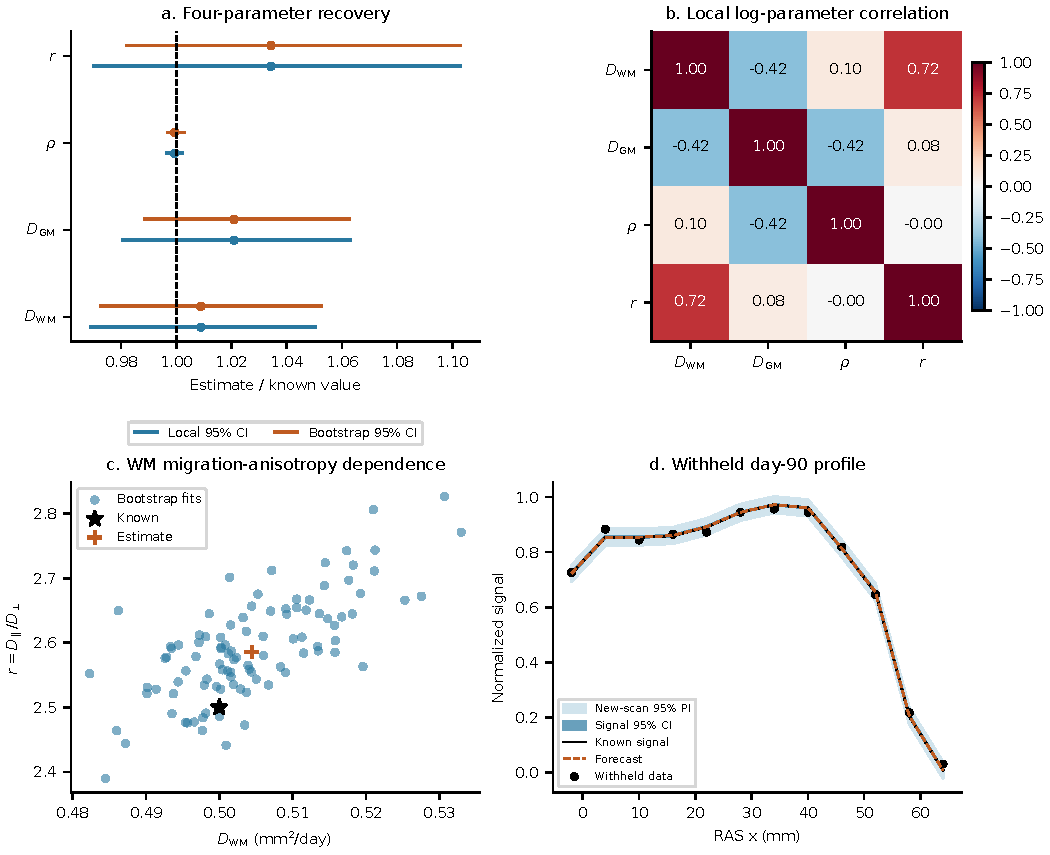
\includegraphics[width=\textwidth]{figures/pat16_recovery.pdf}
\caption{PAT16 synthetic recovery and uncertainty. (a) Primary estimates divided by the known generating values, with local and bootstrap marginal 95\% confidence intervals; the dashed line denotes truth. (b) Local log-parameter correlations. (c) All \PRBootstraps{} bootstrap WM-diffusivity/anisotropy pairs, with known values and the primary estimate. (d) A fixed central observation-voxel row at withheld day 90, showing nominal pointwise 95\% signal confidence and Gaussian-mixture new-measurement prediction intervals. The observation row uses $y=\PRProfileY$, $z=\PRProfileZ$ mm in RAS coordinates. No later measurement enters fitting or resampling. The joint dependence should be propagated; separate marginal endpoints do not define independent parameter combinations.}\label{fig:pat16_recovery}
\end{figure}

Across \PRTrials{} independent noise datasets, marginal local-interval coverage was \PRWhiteCoverage/\PRTrials{}, \PRGrayCoverage/\PRTrials{}, \PRRhoCoverage/\PRTrials{} and \PRRatioCoverage/\PRTrials{} (Table~\ref{tab:pat16_recovery_coverage}; Figure~\ref{fig:pat16_recovery_validation}). Mean relative biases were $\PRWhiteBias\%$, $\PRGrayBias\%$, $\PRRhoBias\%$ and $\PRRatioBias\%$. Exact binomial intervals contained the nominal 95\% level but remained broad; this is not evidence of established 95\% calibration. The audit includes the declared temporal mismatch while holding anatomy, directions, initialization and observation calibration fixed. It does not assess marginal bootstrap parameter-interval coverage or robustness to broader model error.

\begin{table}[tbp]
\centering\small
\caption{PAT16 independent-noise audit of local 95\% intervals. Bias is relative to the known parameter; RMSE uses the parameter's units. Exact binomial intervals quantify Monte Carlo uncertainty in coverage. Failed/boundary intervals would count as misses; none occurred.}\label{tab:pat16_recovery_coverage}
\setlength{\tabcolsep}{3pt}
\begin{tabularx}{\textwidth}{lrrYY}
\toprule Parameter & Mean bias & RMSE & Local coverage & Exact 95\% binomial CI\\\midrule
\PRCoverageRows
\bottomrule
\end{tabularx}
\end{table}

\begin{figure}[p]
\centering
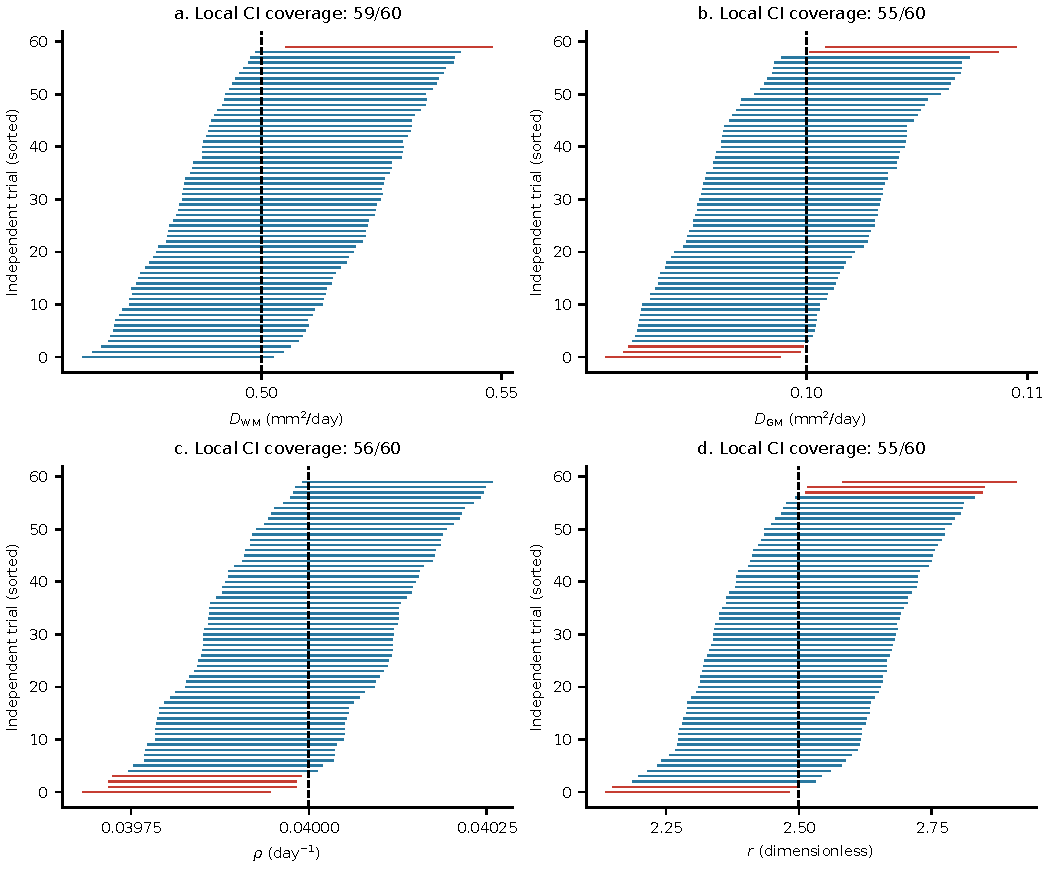
\includegraphics[width=\textwidth]{figures/pat16_recovery_validation.pdf}
\caption{Validation against known synthetic generating parameters on PAT16 anatomy across \PRTrials{} fresh noise datasets. Each segment is a marginal local 95\% interval, sorted within parameter by fitted value; the black dashed line is the known value. Red intervals miss truth. Counts include all attempted trials. These repetitions share anatomy, initialization, directions, biology and observation calibration; they are independent noise realizations, not independent patients. Exact binomial intervals and parameter bias/RMSE are reported in Table~\ref{tab:pat16_recovery_coverage}.}\label{fig:pat16_recovery_validation}
\end{figure}

\subsection{PAT16 withheld forecasts and numerical validation}\label{sec:pat16_recovery_forecast}
Full-cube forecast RMSE against the noise-free signal was \PRDaySeventyFiveRMSE{} at day 75 and \PRDayNinetyRMSE{} at day 90, while noisy-scan RMSE was approximately the assumed 0.015 noise standard deviation (Table~\ref{tab:pat16_recovery_forecast}). The nominal pointwise 95\% signal intervals contained \PRDaySeventyFiveSignalContainment\% and \PRDayNinetySignalContainment\% of full-cube truth values. Final Gaussian-mixture prediction intervals contained \PRDaySeventyFivePredictionContainment\% and \PRDayNinetyPredictionContainment\% of noisy observations; near-center fractions were \PRNearDaySeventyFivePredictionContainment\% and \PRNearDayNinetyPredictionContainment\%. These descriptive spatial fractions do not establish repeated or simultaneous coverage.

Mean full-cube signal-interval widths were \PRDaySeventyFiveSignalWidth{} and \PRDayNinetySignalWidth{}; final prediction widths were \PRDaySeventyFivePredictionWidth{} and \PRDayNinetyPredictionWidth{} normalized signal units at days 75/90. The original 100 noisy draws gave about 93.2\%/93.1\% containment and widths 0.05642/0.05639. Increasing predictive draws to 1,000 and \PPDraws{} reduced interval-endpoint RMSE against the integrated mixture from \PPEndpointLegacy{} to \PPEndpointThousand{} and \PPEndpointMany{}, respectively (Figure~\ref{fig:pat16_prediction_validation}a). Integration removes noise-tail sampling error without tuning widths; the number of distinct parameter vectors remains \PRBootstraps{}.

\begin{table}[tbp]
\centering\small
\caption{Withheld PAT16 forecast validation. The full FOV contains 1,728 observation voxels and the near-center sphere 280. Signal RMSE is against noise-free truth. The noisy RMSE is divided by the known noise SD. The last two columns report spatial containment in nominal pointwise 95\% signal confidence and Gaussian-mixture new-observation prediction intervals, respectively. These fractions are not an independent coverage audit.}\label{tab:pat16_recovery_forecast}
\setlength{\tabcolsep}{3pt}
\begin{tabularx}{\textwidth}{rlYYYY}
\toprule Day & Region & Signal RMSE & Noisy RMSE/SD & Truth in signal CI & Data in prediction interval\\\midrule
\PRForecastRows
\bottomrule
\end{tabularx}
\end{table}

Across \PPTrials{} independently regenerated datasets and \PPNestedFits{} nested bootstrap refits, full-cube mean coverage was \PPOldFullSeventyFive\%/\PPOldFullNinety\% for 100 noisy draws, \PPManyFullSeventyFive\%/\PPManyFullNinety\% for \PPDraws{} draws and \PPMixFullSeventyFive\%/\PPMixFullNinety\% for integrated intervals at days 75/90 (Table~\ref{tab:pat16_prediction_validation}). The integrated mean-coverage Monte Carlo 95\% intervals were \PPMixFullSeventyFiveCI\% and \PPMixFullNinetyCI\%; near-center mean coverage was \PPMixNearSeventyFive\% and \PPMixNearNinety\%. Day-75 full-cube coverage was slightly conservative: its Monte Carlo lower limit lay just above 95\%, rather than demonstrating exact nominal calibration. Paired full-cube coverage gains over 100 noisy draws were \PPGainSeventyFive{} percentage points (MC 95\% interval \PPGainSeventyFiveCI{}) and \PPGainNinety{} (\PPGainNinetyCI{}) at days 75/90. Widths and interval scores distinguish improvement in tail estimation from point accuracy, which is shared by the methods.

Every primary and nested fit succeeded without a boundary optimum. At the prespecified central voxel, integrated intervals covered \PPSentinelSeventyFive/\PPTrials{} and \PPSentinelNinety/\PPTrials{} fresh observations, with exact binomial 95\% limits \PPSentinelSeventyFiveCI\% and \PPSentinelNinetyCI\%. These broad limits leave single-voxel calibration uncertain. Regional averages support near-nominal pointwise coverage for this fixed design; coverage at each location, under model error or in patients remains unestablished.

\begin{table}[p]
\centering\small
\caption{Repeated PAT16 prediction-interval validation. Each of \PPTrials{} independent datasets refits the four rates and 100 bootstrap samples. Coverage is the mean within-image fraction; bracketed 95\% Monte Carlo limits use dataset-level Student-$t$ uncertainty, avoiding pooled-voxel independence. Width and the proper interval score are in normalized signal units; lower score is better. The score adds $2/0.05$ times the distance of an observation outside the interval to its width. All attempted datasets are included.}\label{tab:pat16_prediction_validation}
\setlength{\tabcolsep}{3pt}
\begin{tabularx}{\textwidth}{lrlYrr}
\toprule Method & Day & Region & Coverage [MC 95\% CI] (\%) & Width & Score\\\midrule
\PPValidationRows
\bottomrule
\end{tabularx}
\end{table}

\begin{figure}[p]
\centering
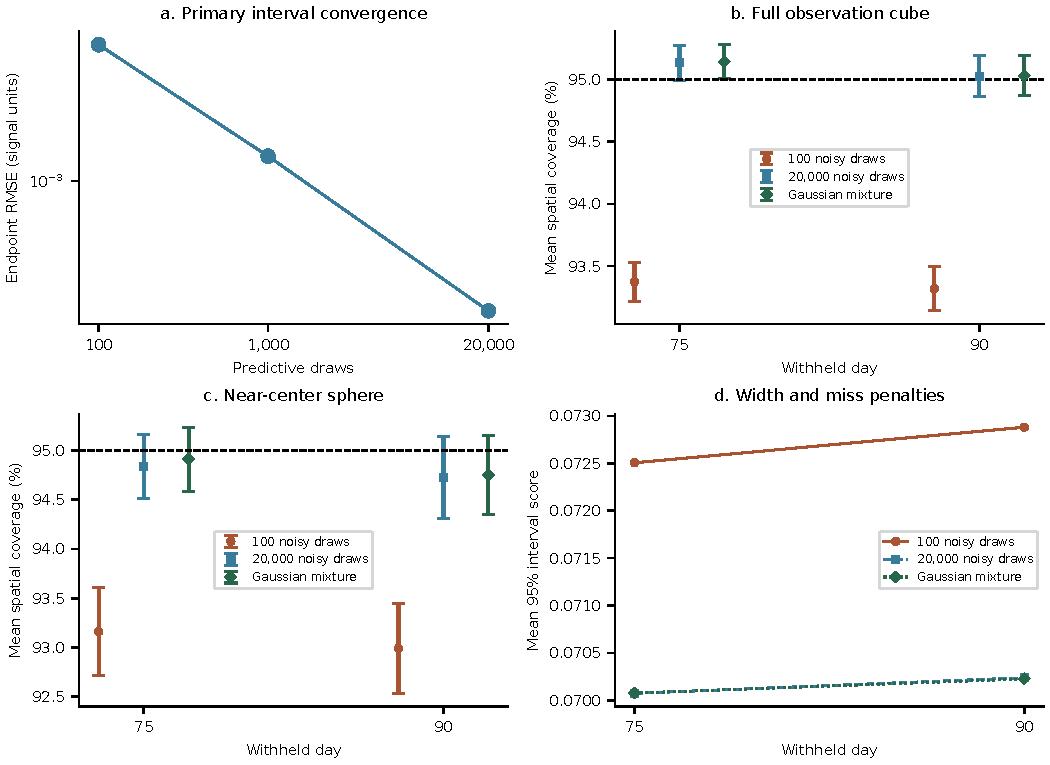
\includegraphics[width=\textwidth]{figures/pat16_prediction_validation.pdf}
\caption{Improved PAT16 pointwise 95\% prediction intervals. (a) Primary endpoint RMSE relative to Gaussian-mixture quantiles, over both tails, withheld days and all observation voxels; 100 draws use the legacy construction, while 1,000/20,000 draws resample bootstrap trajectories. (b,c) Mean spatial coverage across \PPTrials{} fresh datasets, with dataset-level Monte Carlo 95\% limits; the dashed line is nominal coverage. (d) Mean full-cube proper interval score, penalizing width and misses. Each repetition independently refits the early data and 100 bootstrap datasets; future noise is independent of training and resampling. Gaussian integration removes predictive noise sampling error, while uncertainty from finite bootstrap fits and the fixed model remains.}\label{fig:pat16_prediction_validation}
\end{figure}

The noise-free matched-model fit recovered all four generating values with maximum relative error \PRMatchedError{}; this is a matched-discretization implementation check. Fitting noise-free finer-time signals shifted WM diffusion, GM diffusion, proliferation and anisotropy by $\PRWhiteTemporalShift\%$, $\PRGrayTemporalShift\%$, $\PRRhoTemporalShift\%$ and $\PRRatioTemporalShift\%$, respectively. Thus the largest temporal-mismatch shift was \PRTemporalMaxShift\%. These deterministic shifts are outside the sampling-interval construction. The check retained the spatial anatomy and stencil and cannot establish spatial convergence. Time-zero-only inference was correctly rejected. Tests also rejected four-parameter fitting without directional information or with only one tissue class. Conditional numerical recovery and synthetic forecasting do not validate the patient observation model or biological migration anisotropy.

\begin{figure}[p]
\centering
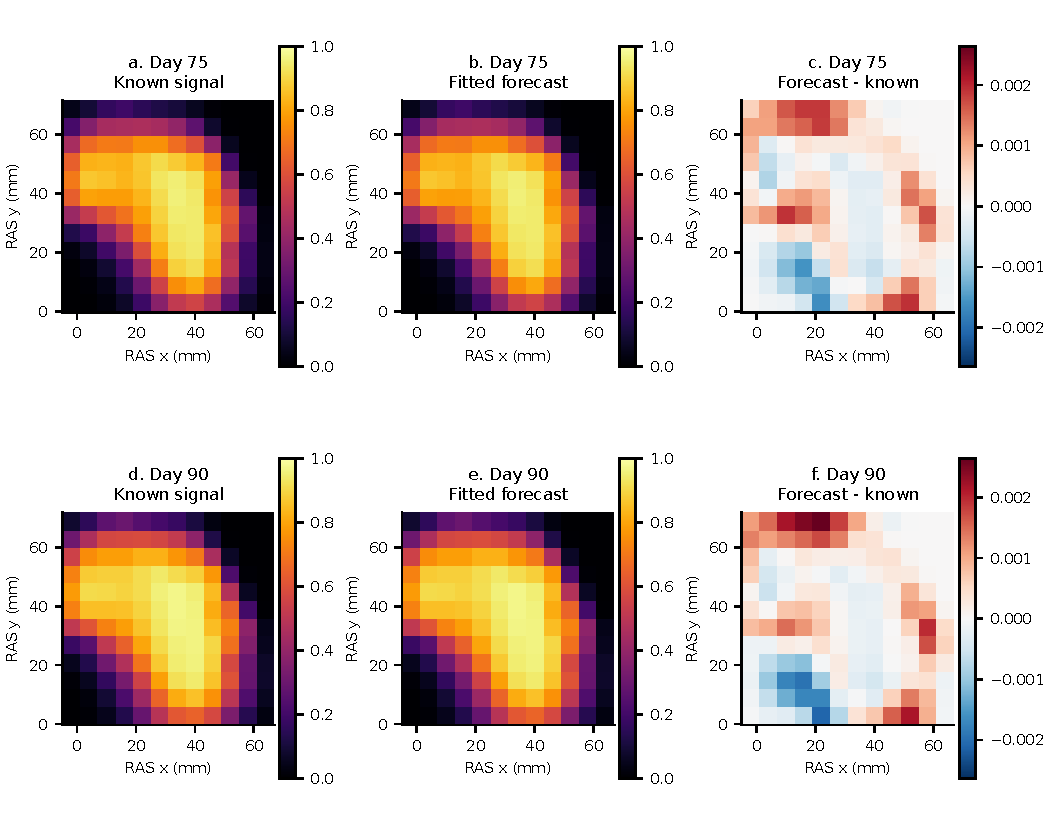
\includegraphics[width=\textwidth]{figures/pat16_recovery_forecast.pdf}
\caption{PAT16 withheld day-75 (top) and day-90 (bottom) noise-free signals on the central observation plane, RAS $z=\PRProfileZ$ mm. Left: known synthetic signal. Middle: the forecast calibrated only at days 20/40/60. Right: fitted minus known signal, with one shared symmetric residual range retaining all displayed errors. The known and fitted signals share a $0$--$1$ scale. Each pixel approximates a 6 mm cube average after Gaussian blur with 2 mm standard deviation; these are synthetic signals, not patient MRI intensities or a fine-grid tumor-density slice. Pointwise interval behavior is shown in Figure~\ref{fig:pat16_recovery}d and Table~\ref{tab:pat16_recovery_forecast}.}\label{fig:pat16_recovery_forecast}
\end{figure}
\FloatBarrier
